\section{Blockschaltbild und Automatengraph}

% grafik einbinden
\begin{figure}[H]
    \begin{center}
        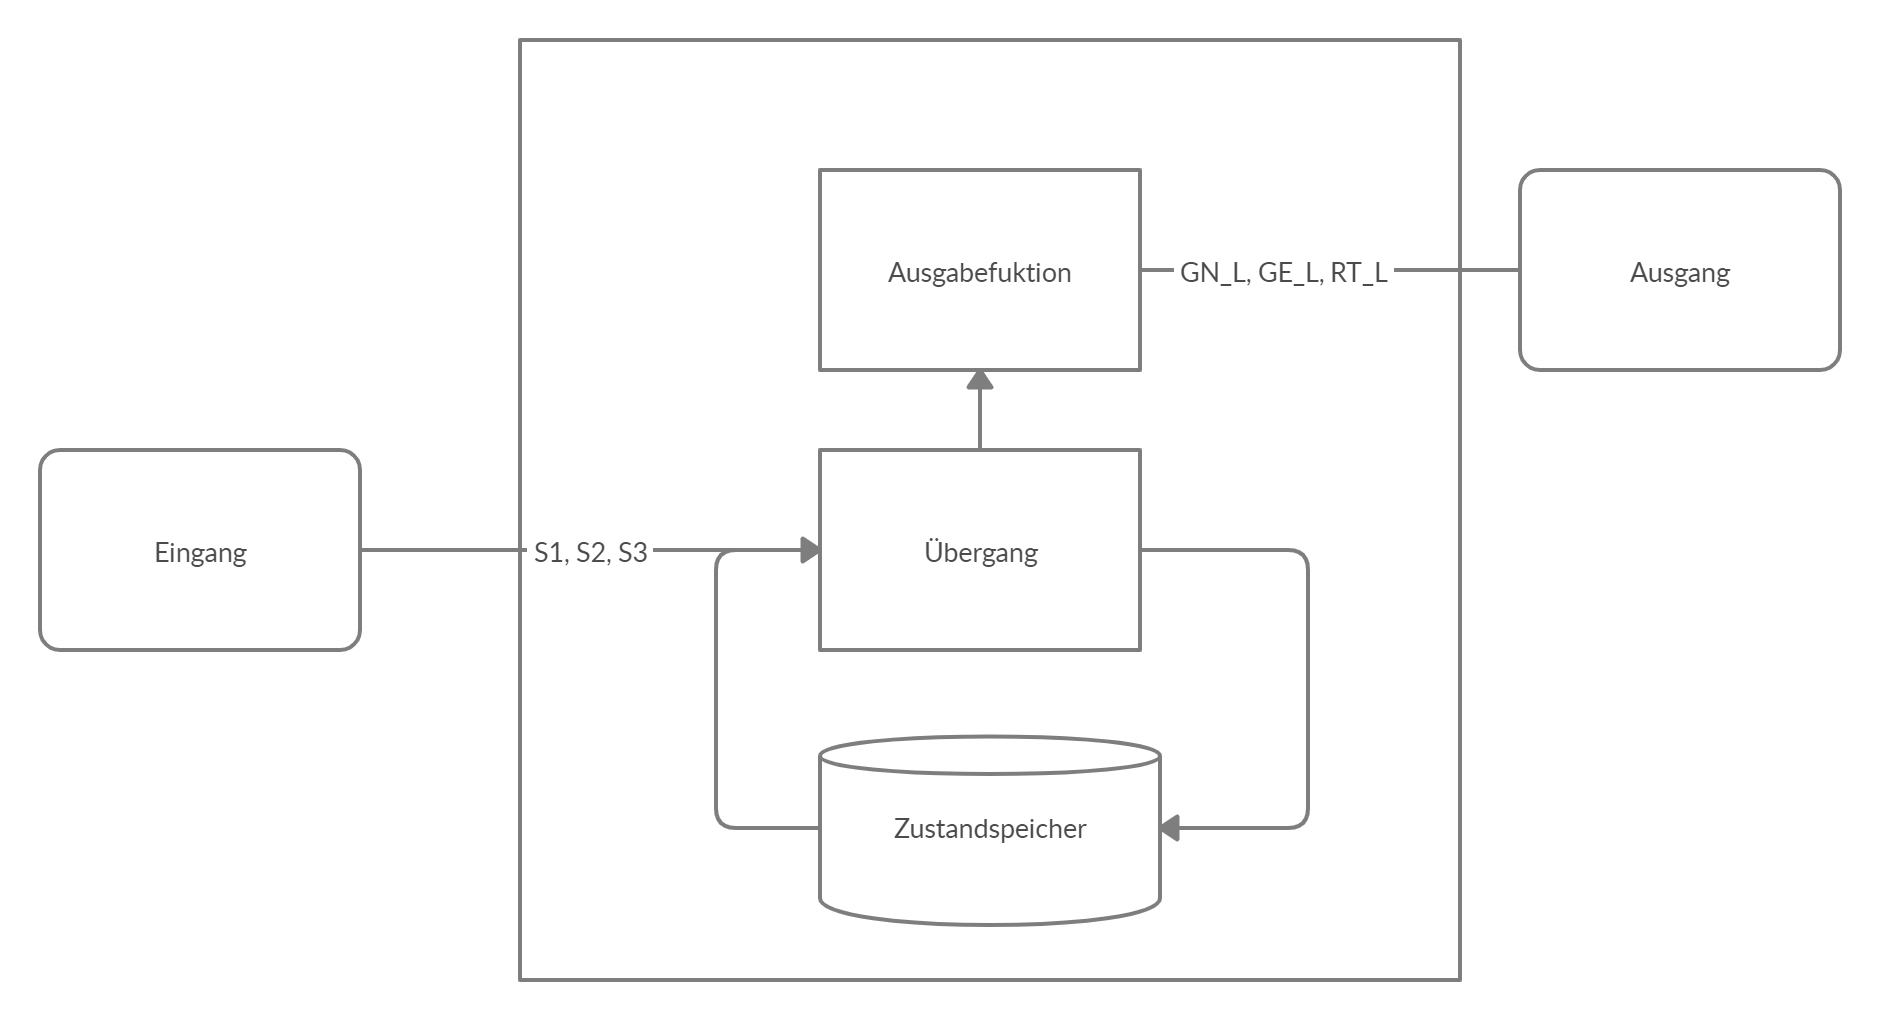
\includegraphics[width=0.8\textwidth]{img/Blockschalt.png}
        \caption{Blockschalt}
        \label{fig:A1_Block}
    \end{center}
\end{figure}


% grafik einbinden
\begin{figure}[H]
    \begin{center}
        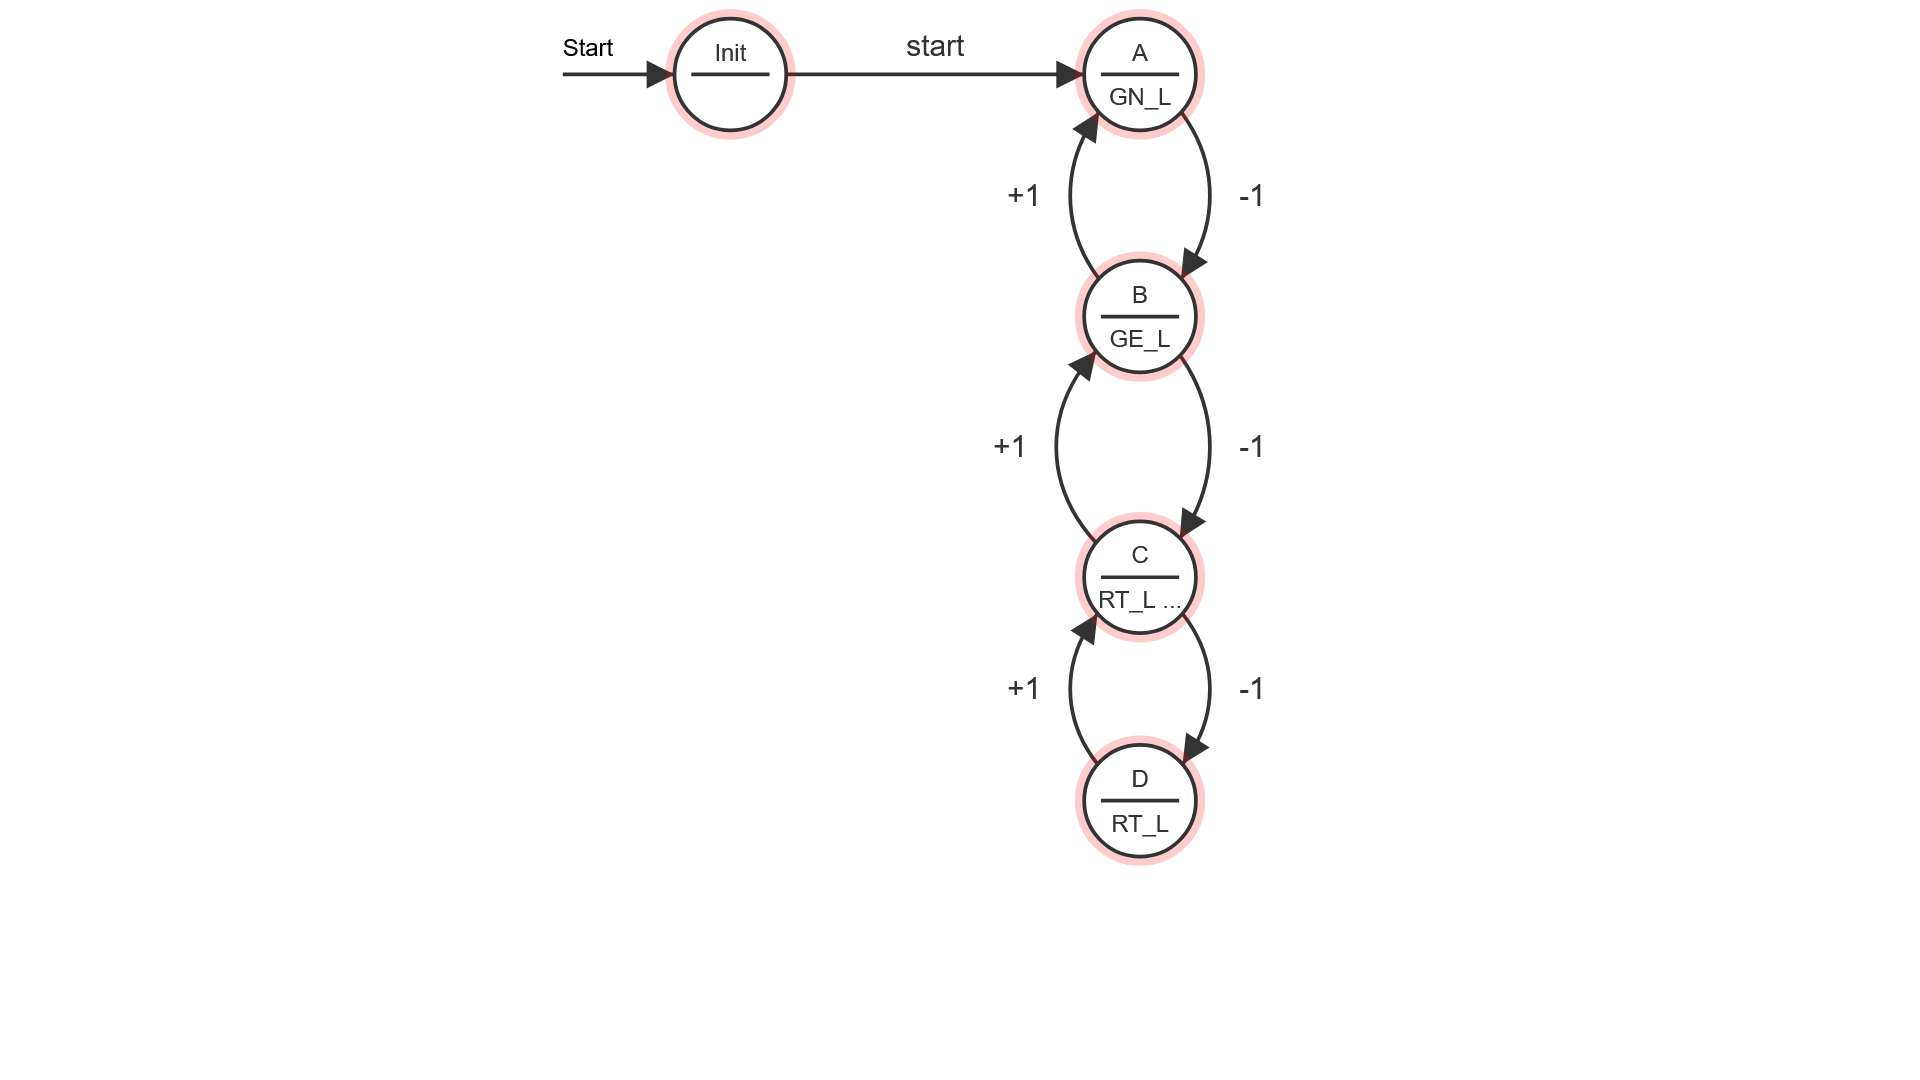
\includegraphics[width=0.8\textwidth]{img/Motortemp.png}
        \caption{Automatengraph}
        \label{fig:A1_Auto}
    \end{center}
\end{figure}
Tupel des Automaten:
Zustände:
\[Q =\{Init, A, B, C, D\}  \]
\[mit \ q_0 = Init \]\\
Eingabealphabet:
\[\Sigma =\{0,1,2,3\} \]\\
Ausgabealphabet:
\[\Omega = \{GN\_L, GE\_L, RT\_L\} \]\\
Ausgabefunktion:
\[\lambda = \lambda  : Q \Rightarrow \Omega: \]
\[  \lambda:GN\_L \Rightarrow \Sigma <= 3 \]
\[  \lambda:GE\_L \Rightarrow 0 < \Sigma <= 2  \]
\[  \lambda:RT\_L \Rightarrow  \Sigma <= 1  \]\\

 Automaten Tafel:\\
 \begin{table}[ht]
    \centering
    \begin{tabular}{|c|c|c|c|c|c|c|}\hline
    \tbf{$\delta$ (Übergang) $\searrow$} & \tbf{$\Sigma= 0$} & \tbf{$\Sigma= 1$}  & \tbf{$\Sigma= 2$} & \tbf{$\Sigma= 3$} & \tbf{$\Delta$ (Ausgabe)} \\ \hline
    $q_0$ = Init    & D     & C     & B     & A     & GN\_L, GE\_L, RT\_L   \\
    A       & D     & C     & B     & A     & GN\_L                 \\ 
    B       & D     & C     & B     & A     & GE\_L                 \\ 
    C       & D     & C     & B     & A     & GE\_L + RT\_L         \\ 
    D       & D     & C     & B     & A     & RT\_L                 \\ \hline
    \end{tabular} 
    \caption{Beispiel Addieren:}
\end{table}



Das Eingangstupel besteht aus dem Signal der Sensoren der Pumpen. Der Übersichtlichkeit her wurde auf dem Graph nur modelliert, dass eine pumpe ausfallen oder wieder funktionieren kann. \(\Sigma =\{-1,+1\} \)
 Der Automat kann Zustände auch überspringen, wenn z.B. zwei pumpen gleichzeitig ausfallen, dies wurde zwecks Übersichtlichkeit nicht eingezeichnet.\\
 


\subsection{Aufbau}

\subsection{Durchführung}

\subsection{Auswertung}
